\subsection{Communication Message Broker}

A communication framework supports our hierarchical job model
by establishing a {\em comms session} to contain each \flux instance
and provide a foundation for the distributed components upon which
\flux\ is built.
This framework enables secure, scalable communication
within a comms session, limits communication between sessions,
and allows new comms sessions to be created, resized, destroyed,
and monitored by existing ones in a parent-child relationship.
The framework is persistent for the life of a job and is anticipated to be
shared among \flux\ services, tools, and application runtimes.

\begin{figure}
\centering
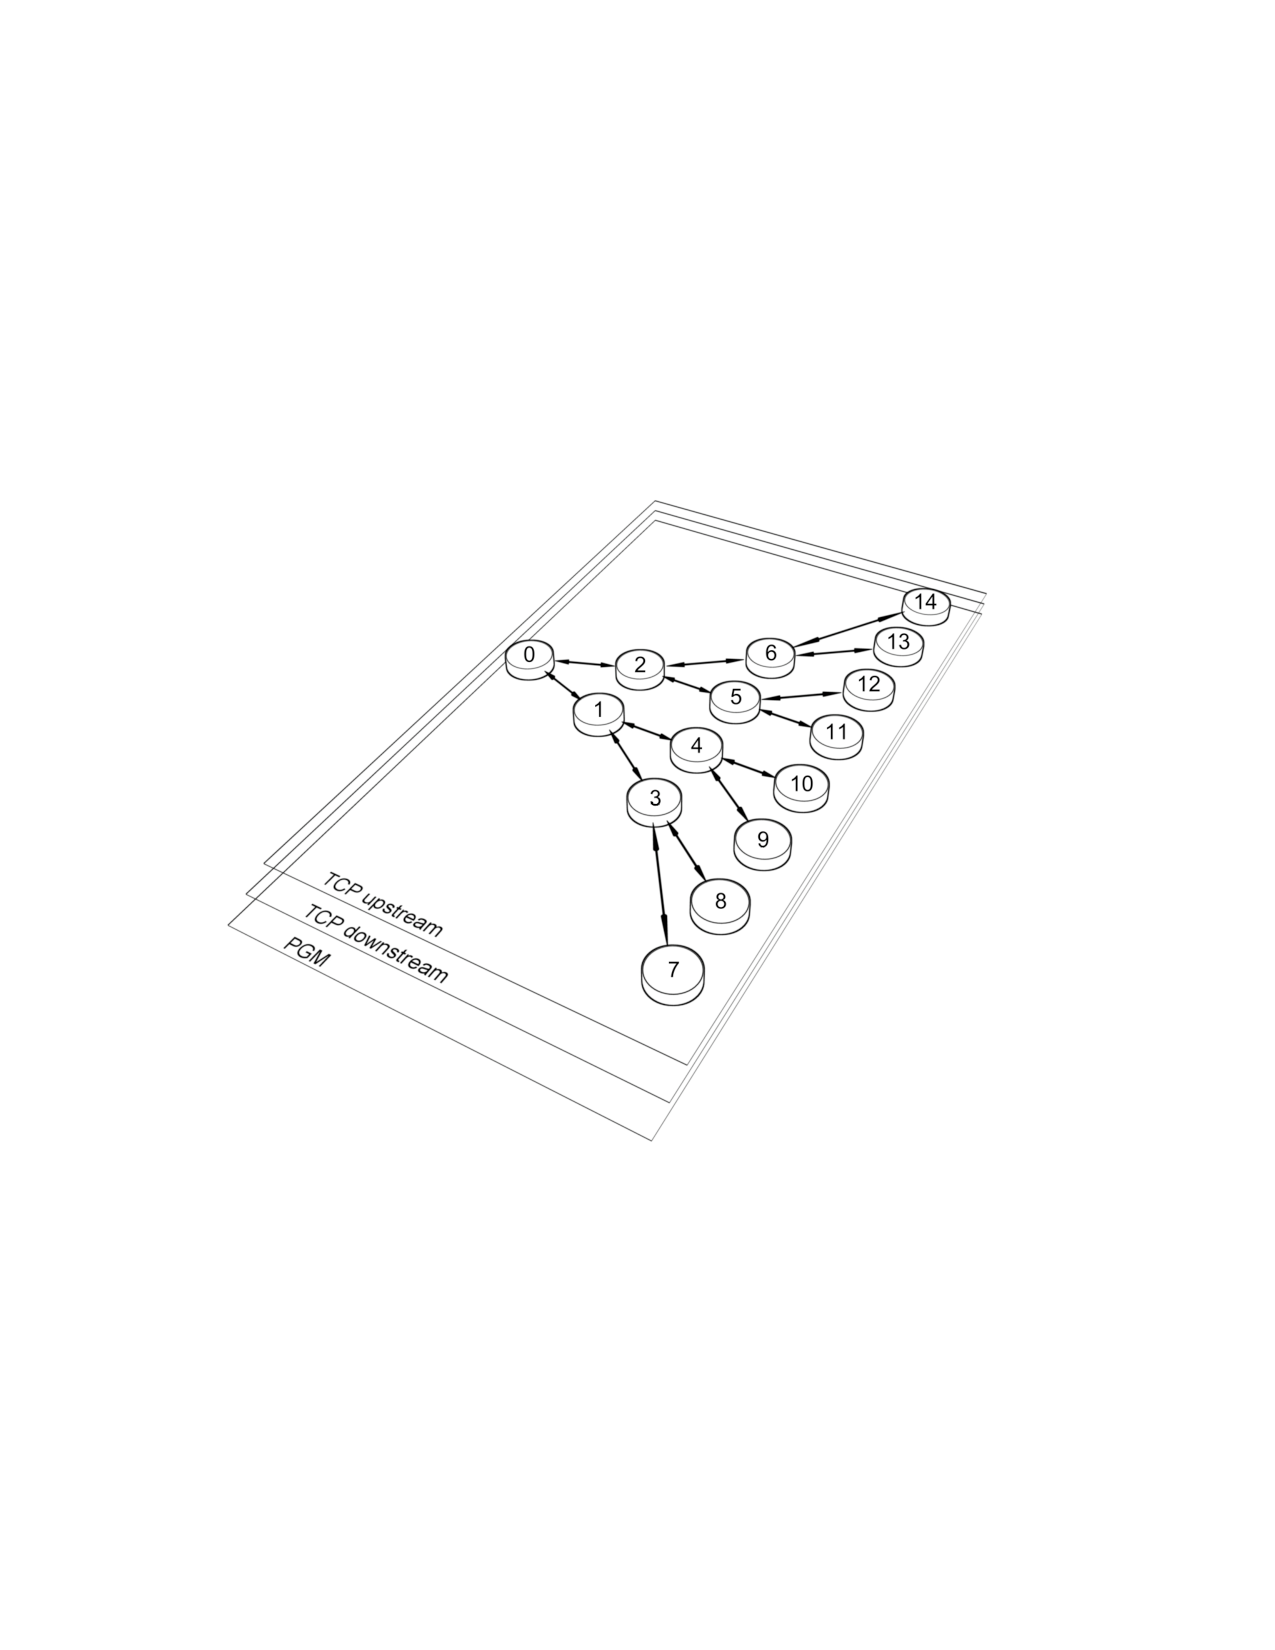
\includegraphics[trim=5.0cm 8.0cm 5.0cm 8.0cm,scale=0.45]{B_Tree_4Layer_BW}
\vspace{-.3cm}
\caption{A comms session} 
\vspace{-.5cm}
\label{fig:commswireup}
\end{figure}

We have built a prototype of the framework using the \zMQ~\cite{ZMQGuide}
%which we can launch within a
%Slurm~\cite{Jette02slurm} job.
messaging library, which provides the ability to pass messages securely
over multiple transports, including TCP, UNIX domain IPC, shared memory, and
Pragmatic General Multicast (PGM)~\cite{rfc3208}.
%\zMQ\ can be used to build applications or custom message brokers.
Its socket-like API abstracts common messaging patterns such as
{\em request-reply}, {\em publish-subscribe},
and {\em push-pull}.

Our prototype consists of a distributed Comms Message Broker (CMB)
daemon that runs on each node of a comms session, interconnected using
three persistent overlay network planes:
a PGM {\em publish-subscribe} bus for events and synchronization heartbeats;
a TCP {\em request-response} tree for RPCs and reductions; and
%similar to those enabled by MRNet~\cite{mrnet}; and
a secondary TCP {\em request-response} overlay with configurable topology
for rank-addressed RPCs.

%consists of daemons interconnected using
%three persistent overlay network planes:
%a TCP {\em dealer-router} tree for upstream RPCs and reductions,
%a TCP {\em dealer-router} tree for downstream RPCs, and
%a PGM {\em publish-subscribe} bus for events.
%Although a binary tree is pictured, the RPC planes can be launched in
%any tree shape for testing or to tune performance.
%%Flat, degenerate, {\em k}-ary for several values of {\em k}, and
%binomial have been tested.
%}

The comms session wire-up is depicted in Figure~\ref{fig:commswireup}.
Each message plane implements reliable, in-order message delivery, and
can self-heal when interior nodes fail.
Although a binary RPC/reduction tree is pictured, the tree shape is
configurable.
A design for comprehensive fault tolerance, including root node failure,
is a near-term project activity.

The CMB allows us to experiment with loosely coupled distributed services
that share this message routing framework. Various \flux\ components have
been implemented as {\em comms modules}, plugins which are loaded into the
CMB address space and pass messages over shared memory.
Comms modules currently exist for the components listed
in Table~\ref{tab:cmbmod}.
Each embodies an active topic for study and experimentation.
% by the \flux\ team.

In addition to comms modules, external programs communicate with the CMB
over a UNIX domain socket.  A {\tt flux} utility wraps command line access
to about two dozen modular \flux\ sub-commands, and a custom PMI~\cite{PMI2}
library allows MPI runtimes to access the \flux\ KVS and collective barrier
modules over this transport.

\begin{table}
\centering
\vspace{-.5cm}
% implement basic building blocks for \flux\ and
%potentially other applications.  These are the plugins we have prototyped
%thus far, representing a wide range of design maturity.  Each embodies an
%active topic for study and experimentation by the \flux\ team.}
\begin{tabular}{|l|p{7cm}|}\hline
\textbf{Plugin} & \textbf{Description} \\
\hline
hb & A periodic heartbeat event multicast across the comms
	session synchronizes background activity to reduce scheduling jitter.\\
\hline
live & Each tree node receives heartbeat-synchronized {\em hello}
	messages from its children.  After a configurable number of missed
	messages, a liveness event is issued for a dead child.\\
\hline
log & Log messages are reduced and filtered before being placed in
	a log file at the session root.  A circular debug buffer
	provides log context in response to a fault event.\\
\hline
mon & Lua scripts stored in the KVS activate heartbeat-synchronized sampling.
	Samples are reduced and stored in the KVS.\\
\hline
group & \flux groups define and manage collection of processes that can
	participate in collective operations.\\  
\hline
barrier & Collective barriers provide synchronization across \flux groups. \\
\hline
kvs & A distributed key-value store provides a scalable scratchpad
	for \flux and other tools operating within the comms session.\\
\hline
wrexec & Remote processes can be launched in bulk, monitored,
	receive signals, and have standard I/O captured in the KVS.\\
\hline
resrc & Resources are enumerated in the KVS and allocated
	when the scheduler runs a lightweight job. \\
% LWJ is not introduced
%\hline
%sched & Lightweight job requests are queued in the KVS, assigned
%	resources, and launched. \\
\hline
\end{tabular}
\caption{Prototyped Comms Modules}
\label{tab:cmbmod}
\vspace{-.5cm}
\end{table}

All CMB messages have a uniform, multi-part message format consisting of
at least a {\em header frame} and a {\em JSON~\cite{rfc4627} frame}.
The header frame identifies the message recipient using
a hierarchical name space.  For example, a message sent to {\em kvs.put}
is routed to the {\em kvs} comms module, and internally to its handler
for {\em put}.  The free-form JSON frame contains payload parsed by
the addressed comms module.

RPC requests are routed ``upstream'' to the first comms module that matches
it, possibly traversing CMB nodes.  RPC responses are routed back through
the same set of hops, in reverse.  A comms modules may thus be loaded
at a configurable tree depth to tune its level of distribution
or to conserve node resources for application workloads toward the leaves.
The tree topology of the RPC overlay permits data reductions to be performed by
aggregating and retransmitting upstream requests between instances of
a comms module.

Alternatively, RPC's may be addressed to a specific CMB rank using a
separate overlay, currently utilizing a ring topology which allows
ranks to be trivially reached without routing tables.  The main use
of this addressing mode is in tools for debugging the system,
where the high latency of a ring is preferable to additional complexity.

%This can only raise questions and we need to cut.
%As our designs and prototypes for basic \flux building blocks evolve,
%the CMB evolves to provide necessary services.  For example, the CMB API
%now has both C and Lua~\cite{LuaBook} bindings and a custom event reactor interface in
%response to the experience of 
%%meeting a recent milestone to 
%launching MPI jobs and co-locating distributed debuggers. Some of the building
%blocks built on CMB services are described
%in the next section.
%
%, are independently undergoing design iteration.
%We expect to continue evolving the CMB prototype for several more months until
%our design has reached stability and we build a production-level \flux\ 
%communication framework.
